\documentclass[tikz, border=10pt]{standalone}
\usepackage{pgfplots}
\usepackage{pgfplots}
\usetikzlibrary{backgrounds}
\pgfplotsset{compat=1.18}

\begin{document}
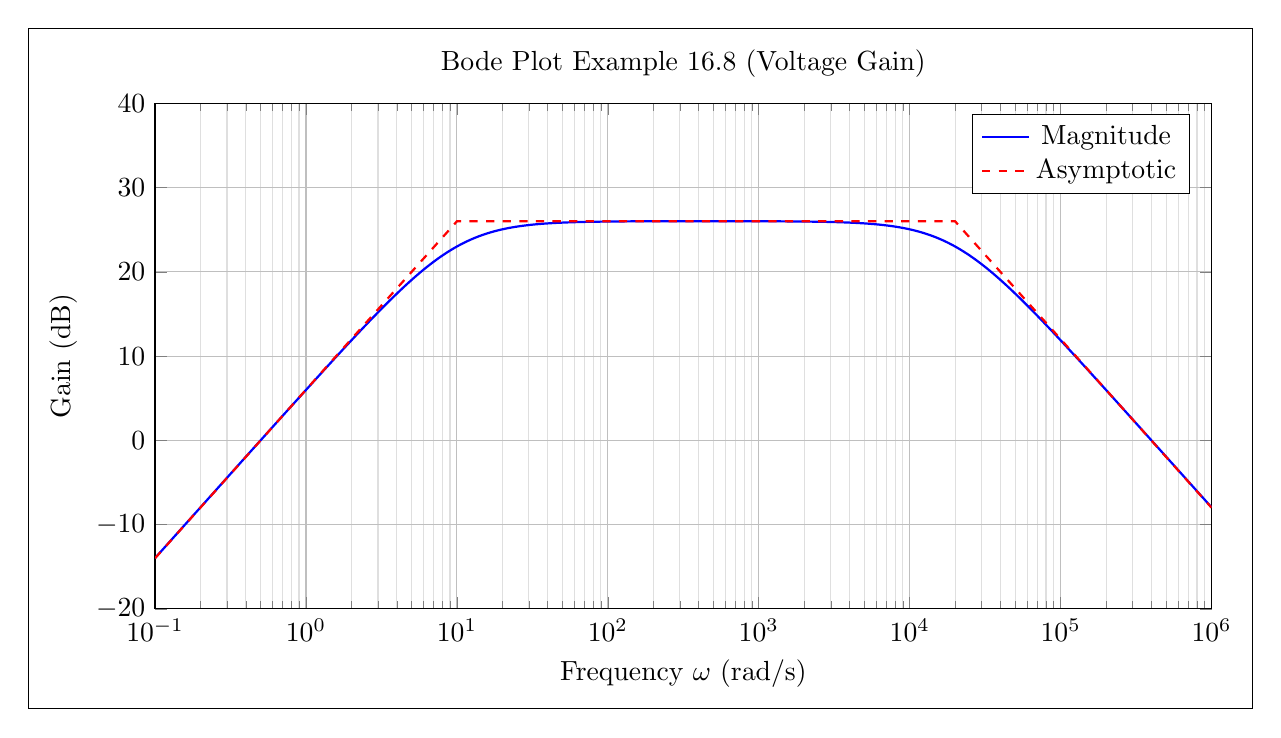
\begin{tikzpicture}[show background rectangle]
    \begin{semilogxaxis}[
        width=15cm, height=8cm,
        title={Bode Plot Example 16.8 (Voltage Gain)},
        xlabel={Frequency $\omega$ (rad/s)},
        ylabel={Gain (dB)},
        grid=both,
        xmin=0.1, xmax=1000000,
        ymin=-20, ymax=40,
        minor grid style={gray!25},
        major grid style={gray!50},
    ]
    % H(s) = -2s / [ (1+s/10)(1+s/20000) ]
    % Magnitude: 20*log10( |-2jw| / ( |1+jw/10| * |1+jw/20000| ) )
    %          = 20*log10( 2*x / ( sqrt(1+(x/10)^2) * sqrt(1+(x/20000)^2) ) )
    
    \addplot[blue, thick, domain=0.1:1000000, samples=300] {
        20*log10( (2*x) / ( sqrt(1+(x/10)^2) * sqrt(1+(x/20000)^2) ) )
    };
    \addlegendentry{Magnitude}
    
    % Asymptotes
    % Low Freq (<10): 20log(2w) -> 0.1: 20log(0.2) = -14dB; 1: 6dB; 10: 26dB
    % Mid Freq (10 < w < 20000): 20log(2*10) = 26dB (Constant, since 2s cancels pole s/10 approx)
    % High Freq (>20000): Slope -20dB/dec
    \addplot[red, dashed, thick] coordinates {
        (0.1, -14) (10, 26) (20000, 26) (1000000, -8)
    };
    \addlegendentry{Asymptotic}

    \end{semilogxaxis}
\end{tikzpicture}
\end{document}
